\label{chap:implementation_ground_station }

The UAV Image Viewer Software is the only application that the user can access to. 
Therefore, the implementation of this program need to include all the specification and also some extra features to make the GUI looks nice.
The plan on making this GUI is to start developing function by function using as much console application as possible such as connect to the port, send/receive information, and change image data to a readable byte.
Upon the final stage of the GUI, the software code runs either in user mode so the user does not has access to the changing of the internal program\cite{tsuiK}. 
This allows a different level of privilege in accessing memory and other system resources. 

The plan of constructing the image viewer is to make a program that the use can simply click on a button and the image is downloaded via TCP/IP port to the ground station.
The programmer make use of both data stream port and the console port in order to send command and receive JPEG photo from the UAV.

\section{The development process} 
Because GUI include many functions on the application and also it links to TCP/IP ports, the GUI part consider as a very big program. 
Therefore, in order to complete the GUI step by step, it needs a plan for the development.
The connection to datastream can be done by using a console application describe in section\ref{sec:testing_connection_send_to_stream}.
If the connection is correct the appliction can listen to the data stream port as in section\ref{sec:testing_receive_stream}.
These console application will be combined to a bigger and more complete program in later section.

\flushleft
\begin{enumerate}


\item	The most important process of GUI development is to understand what does the customer wants. 

\item	The hardware and software specification have to be determined.
 
\item	Make a GUI design decision

\item Develop a smaller program in order to make the testing easy and less time consuming. 

\item	Learn the .NET class that can support the connection to TCP/IP, and communication between host and device

\item	Use GUI to link to the customer’s software to access the software

\item	Distribute the GUI
\end{enumerate}

\section{Use Case Diagram}
The use case diagram show what functionality the user can use in the program.
It has to include all the specification that the customer want for a complete system.
Figure~\ref{GUI_useCase} shows a possible user action on the program which the user can save, open and delete any jpeg image from the computer. 
The user has an option to connect to the UAV in case of the UAV is not connected properly.
He can command the image viewer program to send an image to the software, and it will display the image onto the picture box.
\begin{figure}[H]
\begin{center}
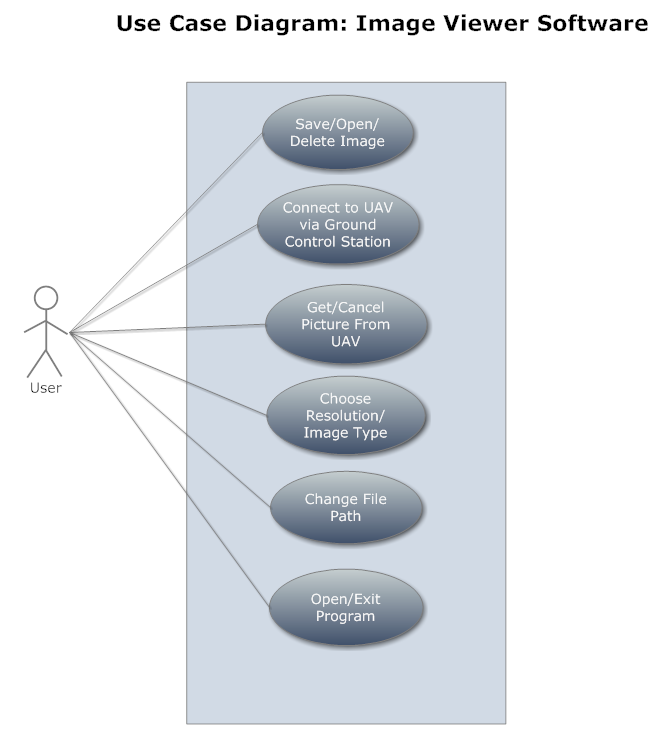
\includegraphics[scale=0.6]{figures/userCase.png} 
\end{center}
\caption{Use case diagram of the GUI\label{GUI_useCase}}
\end{figure}

This initial user diagram has changed because some of the action implement in the background. For example, connect to the UAV function, the user might be confused and click on this button every time the program is open. So the better way to implement this is to make the program connect to the UAV automatically when the program starts running. 
Another changes is the type of image implemented is JPEG only because the raw image will be too big so we decide not to implement it.
Therefore, the Milestone\ref{sec:ms_pl_img_gs_cam_colour_type} will not be implemented.
Figure\ref{GUI_finalUseCase} shows an agreed use case diagram. 

\begin{figure}[!hbtp]
\begin{center}
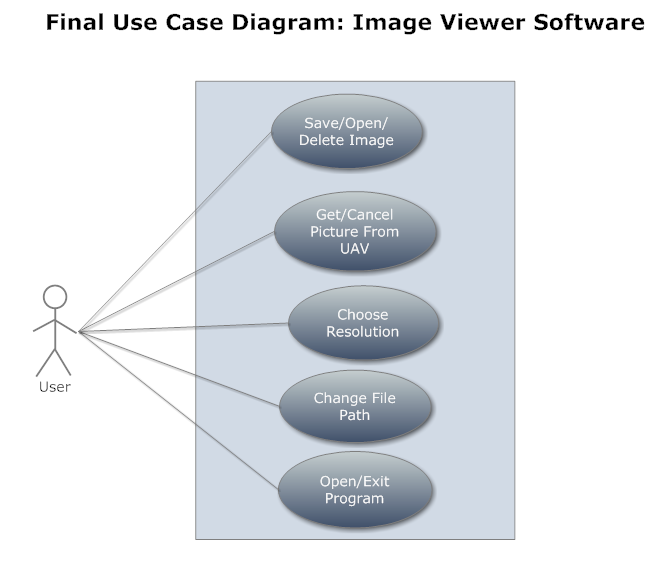
\includegraphics[scale=0.7]{figures/FinaluserCase.png} 
\end{center}
\caption{Final use case diagram of the GUI\label{GUI_finalUseCase}}
\end{figure}



\section{The Design}

The user for our application is assumed to have a limited programming experience, so the program will be implemented so it is simple understand. Figure~\ref{ini_GUI} show the first brainstorm view of the GUI. 

The user interface has a picture box. 
When the user pushes a ‘Get Picture’ button, the picture box will display the picture taken from the UAV. 
During the downloading process, the application should keep running so the cancel button can be used. 
Gallery button will link to another page which will be the collection of images taken. 
Left and right button can navigate the picture box to view an earlier picture or later picture. 
Cancel button cancel the receiving image, therefore the corrupted picture will not be downloaded. 
The user mode of the application can access only the main feature such as take picture, change directory, and cancel download picture.  
It allows the user to choose the resolution and picture type (RAW or JPEG) to transmitted from the UAV to the ground station. But the user doesn't have access to changing the command, changing the receiving data, and any interaction with the UAV because of safety and avoid of any errors. 
\begin{figure}[H]
\begin{center}
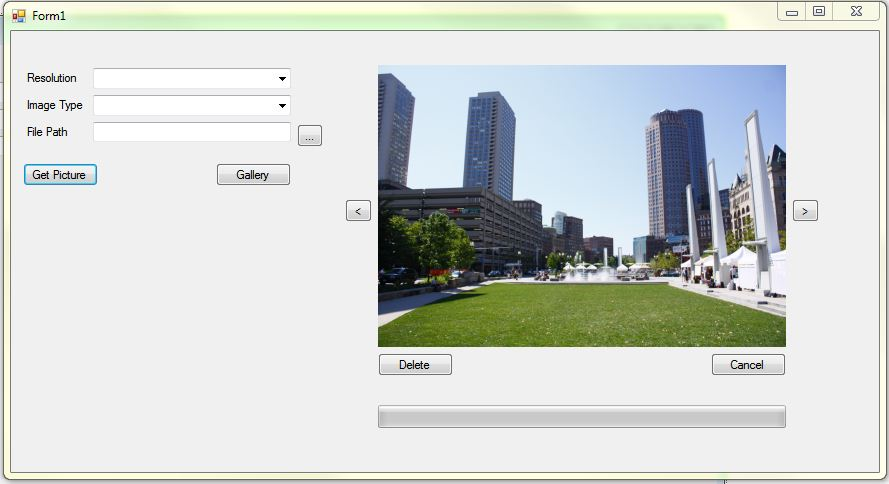
\includegraphics[width=1.0\textwidth]{figures/initialGUI.png} 
\end{center}
\caption{The initial design of GUI\label{ini_GUI}}
\end{figure}
The GUI has been planned to have functions such as auto triggering, image type, resolution type, file path chosen, progress bar, help button, stop and delete. Figure \ref{finalGUI} is the screen shot of the final GUI.

\begin{figure}[H]
\begin{center}
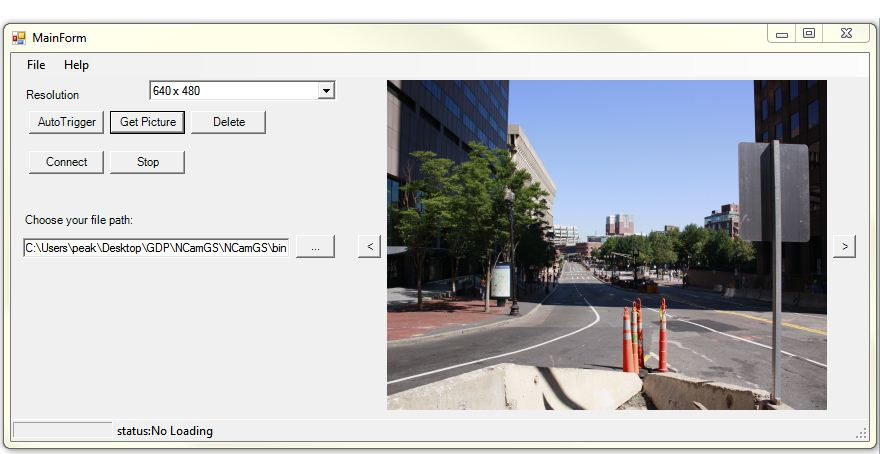
\includegraphics[width=1.0\textwidth]{figures/finalGUI.png} 
\end{center}
\caption{final GUI\label{finalGUI}}
\end{figure}
The top tool strip menu has been added because this layout is familiar to any user. 
The progress bar has moved to the button left of the page instead of displaying it below the pictureBox.
This allows the application to have bigger picture box, more compact size and more professional looks.
The stop button allows the user to interrupt the downloading image.

\section{Class Diagram}
\subsection*{The Initial Class Diagram}
Figure~\ref{ini_Class} shows initial classes and methods of the image viewer program.
The \texttt{JPEGFileReader} Class has functions for decoding/encoding the JPEG file.
There will be decoding/encoding algorithm because the image will take long time to download to the ground station. 
\begin{center}
\begin{figure}[!hbtp]
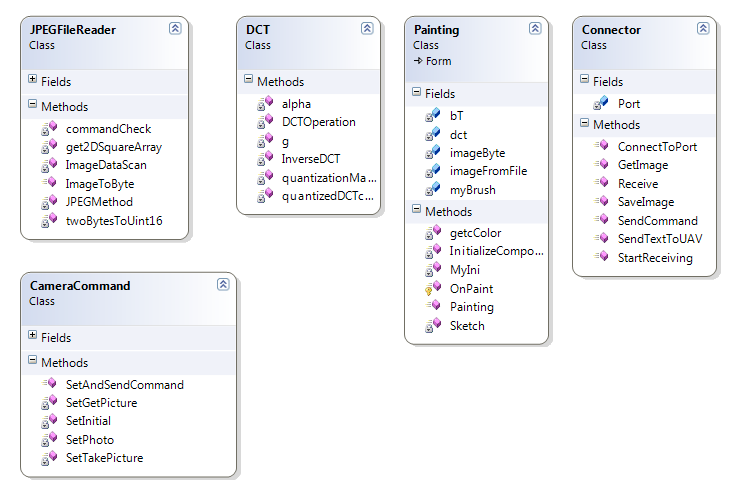
\includegraphics[width=150mm,height=100mm]{figures/initialClassDiagram.png} 
\caption{The initial design of GUI classes\label{ini_Class}}
\end{figure}
\end{center}
\texttt{DCT} class has many math operation and equation which have to be implemented on the image viewer program. 
This complicated function should implement in the ground station because if the picture is encoded in the compressed way, the ground station must be able to extract it. 
In the end, we have to determine whether it is faster to display image normally, or to do encoding/decoding JPEG file. 
The disadvantage of this method is that there are existing encoding resource which work perfectly, and because of this is long length and complex codes.

The \texttt{Painting} class is supported by the \texttt{DCT} class. The intention of this class is to display an encoded image point by point on the \texttt{pictureBox}.
By this method, the \texttt{pictureBox} can display an image from the first pixel transmitted.

The \texttt{CameraCommand} class design for send the data from the ground station to the camera. The idea is that make the camera sync with the payload by using the ground station command. \texttt{SetAndSendCommand()} use for set the byte command and then send it to the payload via the Console port. \texttt{SetGetPicture(),SetInitial(), SetPhoto(), and SetTakePicture()} methods use for setting the correct byte in order to send the byte by using \texttt{SetAndSendCommand} class.

\subsection*{The Class Diagram}
The class diagram has been implemented very differently from the planned one.
This is because the new plan is to decode the image on board and then transmitted to the ground station in JPEG further compressed file. 
Therefore, the class \texttt{JpegFileReader} has changed to C code and to be implemented on board. 
The \texttt{DCT} class is not needed anymore because all the calculation will be on board. 
The \texttt{CameraCommand} has taken away because the payload will receive an image viewer command to the payload and then the payload will send another different signal to the camera.
Therefore, the command send to the camera from the payload does not have to be the same as the command sent from ground station to the payload. 
The \texttt{Painting} class use to draw each pixel onto the \texttt{pictureBox}, but it has not been implemented in the final program because of the stated reason.
The progressive download photo does not have to be implemented. 
Therefore, the milestone\ref{sec:ms_pl_img_gs_progressive_dl} will not be implemented.
This is also because of the time limitation.
More detail about the progressive image is in the section\ref{sec:implementation_progressive_jpeg}.
 
\begin{figure}[!hbtp]
\begin{center}
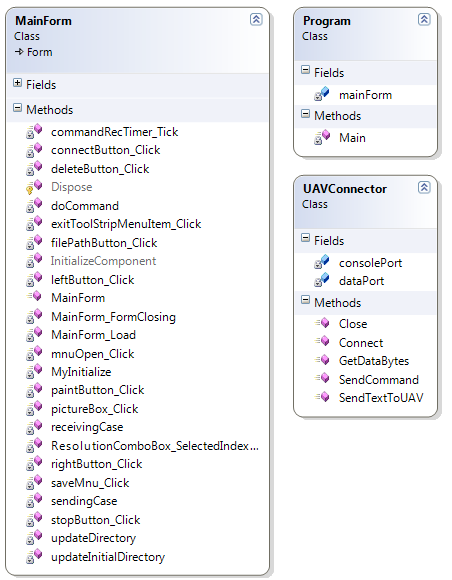
\includegraphics[scale=0.7]{figures/finalClassDiagram.png} 
\end{center}
\caption{Final class diagram of the GUI\label{GUI_finalClassDiagram}}
\end{figure}

\section{Before Connect to the Image Viewer Program}
Figure \ref{schemetic_clipA} shows a diagram of how the connection of the hardware should be. 
The UAV ground receiver is a USB-compatible device which uses Zigbee to communicate. 
USB device driver has been developed by the customer’s so the hardware can be accessed by ground station software, and other applications. 
USB is active when the host ask for a data. 
A host is the computer network which the UAV connect to. 
The data in its queue until the host asks for the data. 
\begin{figure}[!hbtp]
\begin{center}
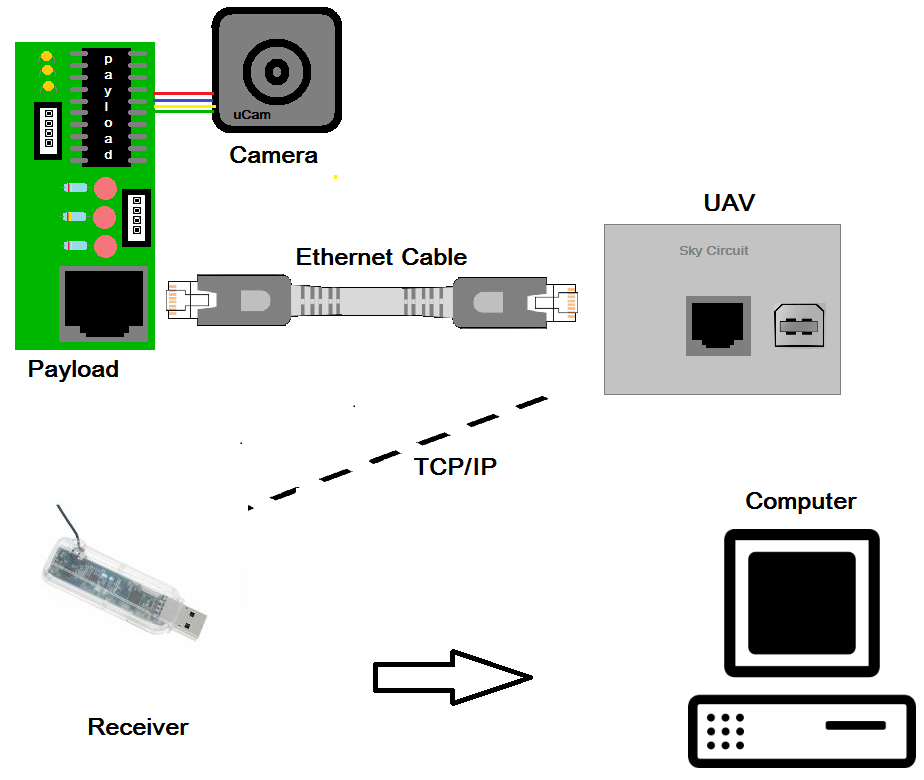
\includegraphics[scale=0.4]{figures/clipArt.png} 
\end{center}
\caption{The connection of the hardware\label{schemetic_clipA}}
\end{figure}


\section{GUI data flow diagram}

Table~\ref{command_table} shows how the command send and receive to/from ground station.  Figure~\ref{GCS_Payload_comm} give a brief detail of how the data communicate between the payload and the image viewer program. 
A more detailed diagram on the data communication is in figure \ref{sequence diagram}.
This has been tested in section\ref{sec:send_console}.

\begin{figure}[H]
\begin{center}
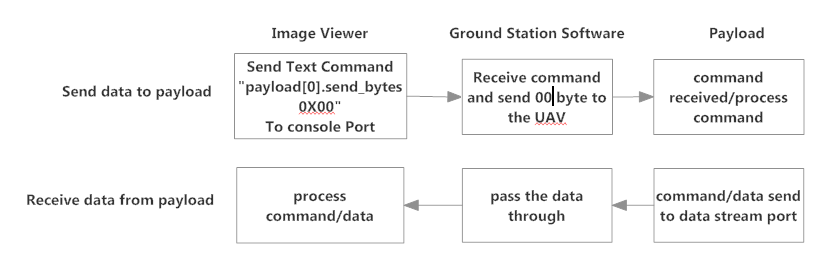
\includegraphics[scale=0.6]{figures/GCS_Payload_communication.png} 
\caption{The connection of data stream port\label{GCS_Payload_comm}}
\end{center}
\end{figure}

\begin{table}[H]

\begin{center}
\begin{tabular}{l l @{.} l}
 Command&
\multicolumn{2}{l}{Address Byte } \\

\hline
\underline{Command from Ground} & \\
SEND\_ZERO\_TOKEN & 0 \\
TAKE\_PICTURE & 0 \\
SEND\_DOWNLOAD\_REQUEST & 2 [MSB] [LSB]  \\
\\
\underline{Command received at Ground}\\
PICTURE\_TAKEN & 1 [MSB] [LSB]\\
DOWNLOAD\_INFO & 3 [MSB] [LSB]\\
IMAGE\_DATA & 4 $\overbrace{ [packet number]}^{2bytes} \overbrace{[image data]}^{data length}$ \\
\end{tabular}
\caption{Command table\label{command_table}}
\end{center}
\end{table}

\section{Get Image Algorithm}
\label{get image algorithm}
In order to take the picture and send it back to the ground station is very important and it has a complex signal algorithm to do.
The plan is when the user click on the Get Picture button, the program sends a \textbf{string command} to the ground station software.
Then the ground station software generates a \textbf{byte command} to transmitted by TCP to the payload. 
Then the payload sends a ''Picture Taken'' command back through the data stream port to the Image Viewer Program. 
Picture taken button has been tested in section\ref{sec:test_get_image_button}
The Image Viewer Program will then automatically send a download request command to the payload. 
The payload will then send image data back to the data stream port. 

When the program start running, the program initialized the port and commands the customer’s application to tell the UAV to stream data to the data stream port. Figure~\ref{GCS_connect_command} shows the connection between the UAV data stream port and the ground station. The UAV has two ports, console port, and data stream port and it can send and receive any length of data. There are some global initializations that the software needs to perform only once when it is loaded for the first time. Note that the console port is manually connected by the ground control station software. The image viewer will give a warning in message box when there is no connection.

\begin{figure}[!hbtp]
\begin{center}
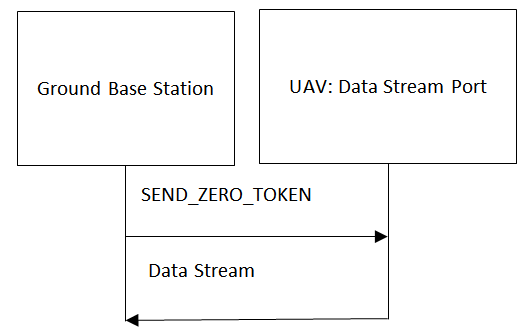
\includegraphics[scale=0.5]{figures/connect_command.png} 
\end{center}
\caption{The connection of data stream port\label{GCS_connect_command}}
\end{figure}

\section{File Dialogue}
For a .NET C\# Programming, there is a previous tools that we can use to change directory, open and save files. The\texttt{OpenFileDialog,  SaveFileDialog, and FolderBrowser} dialogue are existing classes that is suitable to do this job. However, to open any file dialogue, the application needs to have a \texttt{STAThread} in order to handle multiple objects. \texttt{STAThread} is an attribute which applied to the main method, indicating that the application should communicate with unmanaged COM code using the Single Threading Apartment. It allows main thread or the main form to run in the background while the file dialogue is executing. 

These file dialogues are not stated in the image viewer specification. But it has been implemented because the user may install the program in many computers and the initial folder might not exist and this might cause the system to give an error. It is also make the users feel that they can use the program more freely.  It gives the advantage of limiting the access to only an existing file, so there is no error when trying to save the image.

 
\section{Code Highlight}

This section describes the code that is important for the program. The entire code will not be described but it will be in the appendices. It needs a class that can do these to port: connect, receive and send. \texttt{FileStream} class is a class in the .NET C\# which can create a file. \texttt{BinaryWriter} class is use for writing the byte data into a specific file made by the \texttt{FileStream} class. The file directory will introduce a thread. While the open or save a file, the main application must be running, so the application needs to deal with multi threads at the same time. Also when the get picture button got clicked, the main application is frozen because of the thread time organize do one thing at a time. 

\subsubsection*{Connect to UAV:Appendix \ref{appen:UAVConnector} line 18-38.}
The \texttt{Socket} class has functions to send and receive byte and strings data. The handshaking protocol is using \texttt{PortConnect()} method.  
        
The design of the .NET \texttt{Socket} class simply connects to a Port by a single command without any hesitation of changing the baud rate, stop bits, and parity bits. 
This advantage makes the \texttt{Socket} class a more useful class then the \texttt{SerialPort} Class to work with the Port with existing and static set up. 
This class has been tested using a console application before implementing it in a final GUI. 
This will complete milestone\ref{sec:ms_pl_tx_token_resp}.

\subsection{Start of the program: Appendix \ref{appen:main_form} line 78-87}%
In order to make the file name different and meaningful, the name of the picture will be the time and date of the time taken the picture. The code \texttt{DateTime.Now} generate a string of date and time of the current time. This has been done using the date and time class. \texttt{FileStream} was initialize to be in \texttt{FileMode.Create()}, so it can create file. The BinaryWriter write the binary byte into a file in the directory of the fileStream. \texttt{string fileName = string.Format("uavPictureAt{ 0 : yyyy-MM-dd\_ hh-mm-ss-tt}
 .jpg", DateTime.Now);   }  
This code time setting is valid for a file name because it is not using any symbol that will make the program confuse with a code. 
It will display year, month, date, and time in this order. 
The \texttt{BinaryWriter} class can create a binary file using specific data layout for its bytes. 

\subsection{Change File Directory:Appendix \ref{appen:main_form} line346-370 and 454-484 }% 
If the user wishes to change the directory of the image taken, the image viewer program must support it. the mnuOpen\_click() method introduce an OpenFileDialog class. It begins with open file dialog box. This allows the user to open an initial image to the program. If the user took a picture, it will be saved in the same directory as the open file. This file dialog is limited to only the jpg picture in order to avoid the error of displaying the image. 
This file dialog introduces an extra thread. Without thread handler, the program will automatically organize the thread in the same timeline. This means it has to finish one event before it starts another. The more detail about thread will be discussed in the thread section. 

\subsection{Threading}

A Scheduler that is responsible for time-slicing threads controls the thread execution, managing blocking of I/O message and signal handling. There is always a main or initial thread running in a recursive loop that responds to the client application\cite{keithC}. In image viewer program, the main thread is the window application. When the get picture button got clicked, it will generate another less fundamental thread which will be executed after the loop has done. Therefore, in order to deal with this application while the picture is loading we need \texttt{Application.DoEvents();.}
 This code processes all of the Windows event messages that have queued up \cite{davidW}. When this code has been applied, the application can deal with other event at the same time as the code is running. This is important to mention because the program might be stop working if this thread has not introduced.
\texttt{Application.DoEvents()} in the Main function delegate that wraps the method that indicate where to start execution. The thread begin to run when the \texttt{Application.DoEvents()} get called\cite{xieX}.
The \texttt{[STAthread]} has to be introduced in order to run multi thread at the same time. But, this doesn't mean the processor will be faster, but thread can make use of the resources that would go unused. A background thread can continue to run, while a foreground thread waits for the user input. This is called an apartment thread. 
        
\subsection{Text Command:Appendix\ref{appen:UAVConnector} line 68-85}
TCP/IP protocols transfer data without modifying them. This allow the application to freely encode the data.\cite{davidB}.The Ground station software allow the program to send a stream of string in bytes and it will read the command bytes and send it to the payload on the UAV. The code has shown the way to implement the string and send a byte array to the payload.

To send text, the string of characters is translated into an array of bytes. American Standard Code for Information Interchange(ASCII) is use for translating English into a binary code. In the \texttt{System.Text} classes provide converting mechanism between each character sets. The \texttt{ASCIIEncoding.GetBytes()} is used for convert character array into a byte array.  
\texttt{The Socket.Send()} method allows the user to send byte stream to the port connected. The customer's program will read from the port and display it onto the command line. The ''@ '' sign indicate that the command correctly sent from the application to the ground station software. The advantage of linking to the ground station software is that our customers can understand what is going on in the console line. For example:uavConn.SendTextToUAV(''da 20 payload[0].mem\_ bytes[0]'');


The text \texttt{''da 20 payload[0].mem\_ bytes[0]''} will be converted to char array and then to byte array. The byte array will then send the command to the console port to the payload by \texttt{consolePort.Send(toUAVByte, toUAVChar.Length)}. The customer is familiar with the ground station software program, so he can understand the background of the transmission as well. This will complete Milestone\ref{sec:ms_pl_rx_msg_gs}.

In order to test that the payload receives the same data, we use the oscilloscope to see the signal. The byte display on the payload is the same as the byte data send from the ground station. Therefore, the Milesone\ref{sec:ms_pl_img_gs_trigger} is completed. The different resolutions send different byte command to the payload. The byte command changes if the comboBox options change. Therefore, we can say that Milestone\ref{sec:ms_pl_img_gs_cam_res} has completed.

\subsection{I/O Streams}
    The .NET framework's stream class is use as a powerful tool for encoding and decoding\cite{davidB}. In the image viewer program, we use FileStream to create a directory and to save the byte data into image. However, the program might have to deal with a corrupted image data. Framing is the problem of the receiver failed to find the beginning and the end of the message. The solution is the data packet gives the information of how many loop must the program do in order to receive all the image data. The packet address locates in the second and third byte of the image data stream. This will make the completion of Milestone \ref{sec:ms_pl_shared_mem_set}
    
\begin{lstlisting}[caption={writing binary file},label=lst:writingb]          
	for (int i = 3; i < packetSize; i++)
	{
          opFile.Write(packet[i]);
          numBytes++;
    	}
\end{lstlisting}         

At every cycle of the data being received, \texttt{opFile.Write()} method will write the packet data into the file in the directory. After the cycle finished, the file will be saved and the image will be displayed in the picture box. 

\subsubsection*{Update the Directory:Appendix\ref{appen:UAVConnector} line 280-345}
The update directory method updates itself every time the file directory is changing. This method will update the string of the possible JPEG files so when the left or right button got clicked, the string of JPEG file name will get plus or minus and display the next file. This array of string has to update because it changes when the picture got deleted, or the new picture got taken. The array called \texttt{jpegList} is use as string file storage for JPEG file. It has a nice function when the user come to the end of the scrolling up, the right button will disappear, or if it reach the first file in the directory, the left button will disappear. 
\subsection{Get Picture Button}
This get picture button will use both send and receive function of the program. 
The work flow of the get picture signal show in figure \ref{GUI_finalWorkFlow}.
If the sequence of signal send/receive correctly, the photo that receive from the sky will be display on the photo box in the program.
This will complete Milestone\ref{sec:ms_pl_img_sending_gs}.

\begin{figure}[H]
\begin{center}
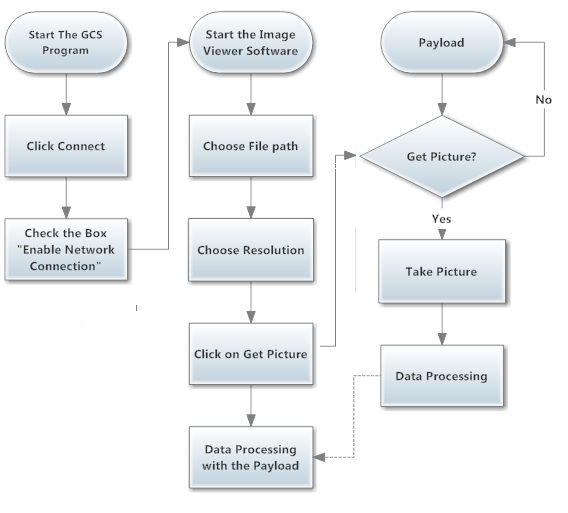
\includegraphics[scale=1]{figures/finalWorkFlow.png} 
\end{center}
\caption{Final work flow diagram of the GUI\label{GUI_finalWorkFlow}}
\end{figure}

\subsection{Implementation - Way-point Triggering (ms)}
\label{sec:waypoint_triggering}

\subsubsection{Description}

The ground station is capable of assigning way-points to
the payload which will allow the camera to take pictures 
at a given location.

This is achieved by sending a simple command script from
the ground station to be uploaded by the payload 
controller. The way-point is designated by the user
through the ground station software. The script 
tells the UAV controller to continuously check the
distance separating itself from the way-point.
When the UAV reaches is within 200 metres of the
way-point, a 0 byte is sent to the camera to prompt
the camera to take a picture.

After taking a picture at the way-point, the camera
is delayed for 10 seconds to avoid taking another picture
at the same way-point. When the 10 second delay is over,
the camera repeats the operation and continuously checks
its distance from the next waypoint.

\subsubsection{Pseudo-code description}

Below is a brief pseudo-code description of the script
sent by the ground station to the payload to take an
image at designated way-points:

\begin{itemize}
	\item while !(UAV distance from next way-point $le$ 200 metres)
		\begin{itemize}
			\item Do nothing.
		\end{itemize}
	\item end while
	\item Prompt camera to take an image.
	\item wait 10 seconds
	\item Re-enter while loop
\end{itemize}

\subsection{Other functions}
The user might want to delete some unwanted photo, so the delete button have been implemented. The delete button work like a normal file deleting button. But it has been complicated because the photo to delete must be the photo on the pictureBox. There is an error because the photo is using by the pictureBox. To fix this problem, the picture have to shifted left or right first and then delete the photo. This will solve almost all the problem. But where there is only one picture in the file, the program is not allow to delete because even the pictureBox is set to null, its last memory is still point at the deleting file. However, the disadvantage of the delete button is that if the wanted photo got deleted accidentally, it might take a long time to launch the UAV again and take the same photo. The program can also detect the corrupted image and ask the user to delete it.

\begin{figure}[H]
\begin{center}
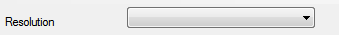
\includegraphics[scale=0.5]{figures/resolutionOption.png} 
\end{center}
\caption{The resolution in combo box\label{resolutionOption}}
\end{figure}
The camera has options of resolution as shown in Figure\ref{resolutionOption}. This can be useful when the speed is important. The lower the resolution, the faster the data transmitted to the ground. GUI has the combo box for the user to choose any wanted resolution in the options. The resolution allow user to have more accessible to the camera. However, this mean there is more on the programmer side to program the application.


The baud rate that we can transmit data from the UAV is 38.4kBaud. Bandwidth limitations severely restrict the volume of data to transfer over the wireless link. It takes around 8 to 20 seconds to transmit an image of resolution 640x480. This progress bar tells the user how much percentage of data received. The progress bar update at each cycle of the data receives. At the end of each image downloaded, the progress bar reset to its normal state.  The status text tells the user what signal have been sent or received. This status text ensures that the picture is downloading and it is good for testing that the tasking in process. These two nice application allocate on the bottom left of the GUI as shown in Figure\ref{progressBar}. However, these have to implement every cycle of the data collection and it might cause the cycle to run slower. The actual loop is much faster than the 38.4kbaud, therefore there is no problem implementing these in.
\begin{figure}[H]
\begin{center}
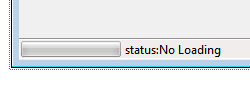
\includegraphics[width=0.3\textwidth]{figures/progressBar.png} 
\end{center}
\caption{The resolution in combo box\label{progressBar}}
\end{figure}

\section{Complete System}
After all the implementation has completed, all the function will be tested together. All the smaller program that we have implemented will be combined at this stage. The send and receiving will use to implement the communication between the payload and the Image Viewer Software. The display of image data will implement as a final display of the image.  Figure \ref{completeSystem} shows a final working GUI of our program. 
\begin{figure}[H]
\begin{center}
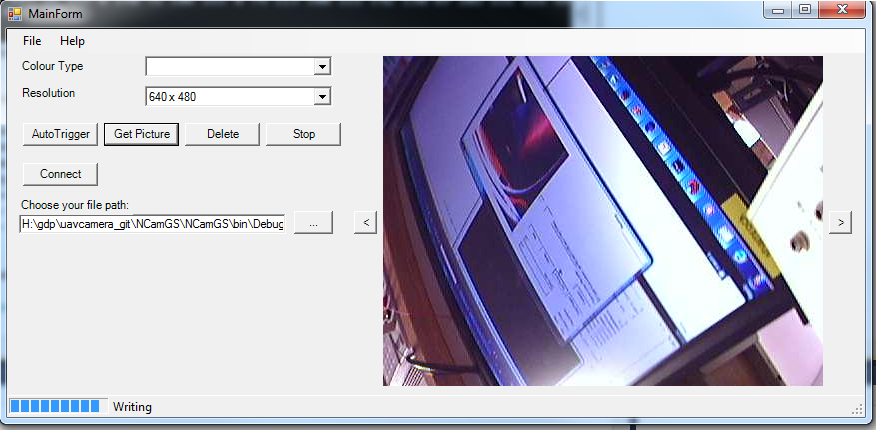
\includegraphics[width=1.0\textwidth]{testing_screenshots/ui.png} 
\end{center}
\caption{The complete system\label{completeSystem}}
\end{figure}


